% This is part of Un soupçon de mathématique sans être agressif pour autant
% Copyright (c) 2015
%   Laurent Claessens
% See the file fdl-1.3.txt for copying conditions.

% This is part of Un soupçon de mathématique sans être agressif pour autant
% Copyright (c) 2015
%   Laurent Claessens
% See the file fdl-1.3.txt for copying conditions.

%--------------------------------------------------------------------------------------------------------------------------- 
\subsection*{Activité : mieux que Thalès ?}
%---------------------------------------------------------------------------------------------------------------------------

À propos du dessin suivant,
\begin{center}
   \input{Fig_GSPNooCOfCGS.pstricks}
\end{center}
Maylis a écrit :
\begin{equation}
    \frac{ A'A }{ OA' }=\frac{ B'B }{ OB' }=\frac{ C'C }{ OC' }
\end{equation}
Est-ce correct ?


\url{interact/cosinus_triple.ggb}

%+++++++++++++++++++++++++++++++++++++++++++++++++++++++++++++++++++++++++++++++++++++++++++++++++++++++++++++++++++++++++++ 
\section{Cosinus}
%+++++++++++++++++++++++++++++++++++++++++++++++++++++++++++++++++++++++++++++++++++++++++++++++++++++++++++++++++++++++++++

D'abord un peu de vocabulaire

\begin{definition}[\cite{NRHooXFvgpp4}]
Dans un triangle rectangle,
\begin{enumerate}
    \item
        l'\defe{hypoténuse}{hypoténuse} est le côté opposé à l'angle droit (c'est le plus long des trois côtés) ;
\item
    le côté \defe{adjacent}{adjacent} à un angle aigu est le côté de cet angle qui n'est pas l'hypoténuse.
\end{enumerate}
\end{definition}

\begin{example}
    Dans le triangle
    \begin{center}
        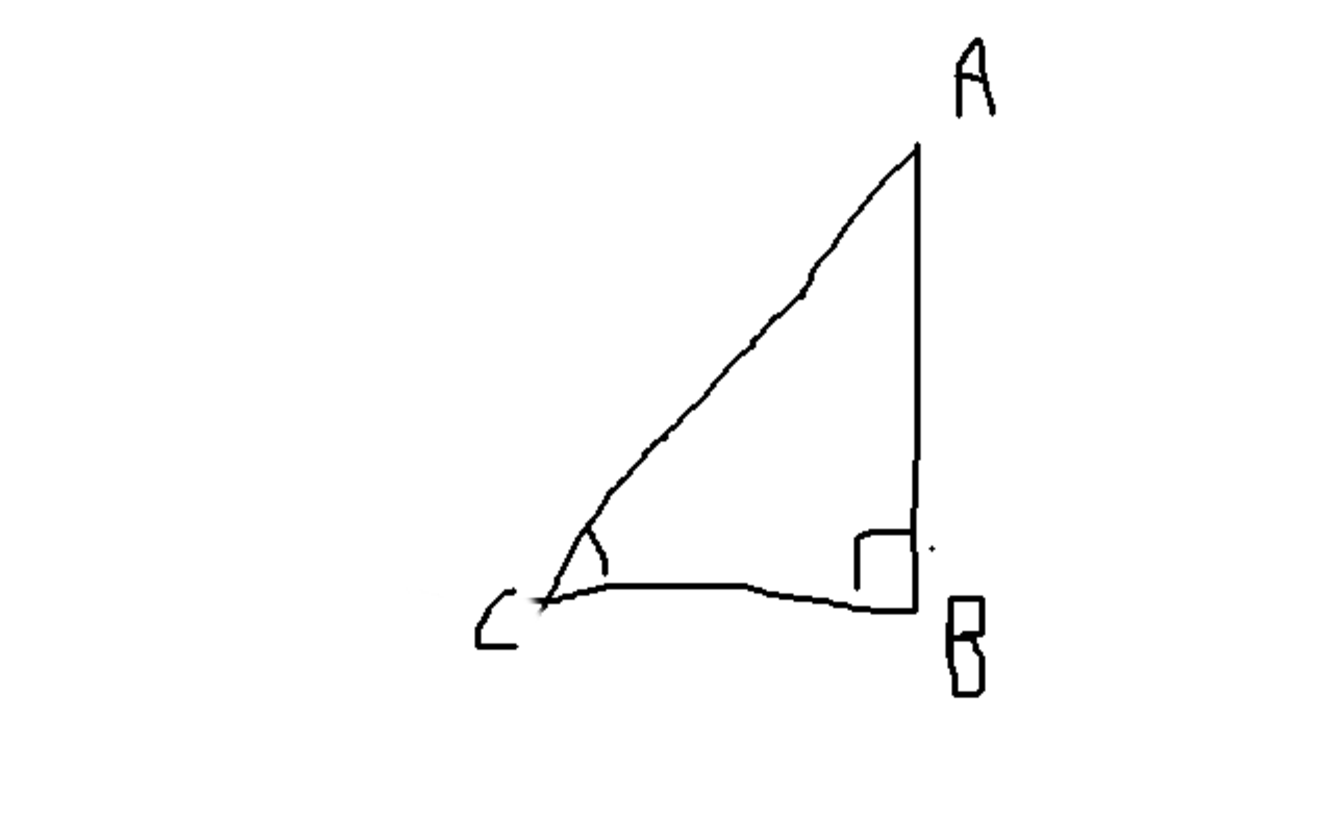
\includegraphics[width=5cm]{faux_ex_adj.pdf}
    \end{center}
    Le côté adjacent à l'angle \( \hat C\) est le côté \( [CB]\).
\end{example}

\begin{definition}[\cite{NRHooXFvgpp4}]
    Dans un triangle rectangle, le \defe{cosinus}{cosinus} d'un angle aigu est le quotient de la longueur du côté adjacent à cet angle par la longueur de l'hypoténuse.
\end{definition}

\begin{example}
    Dans le triangle
    \begin{center}
        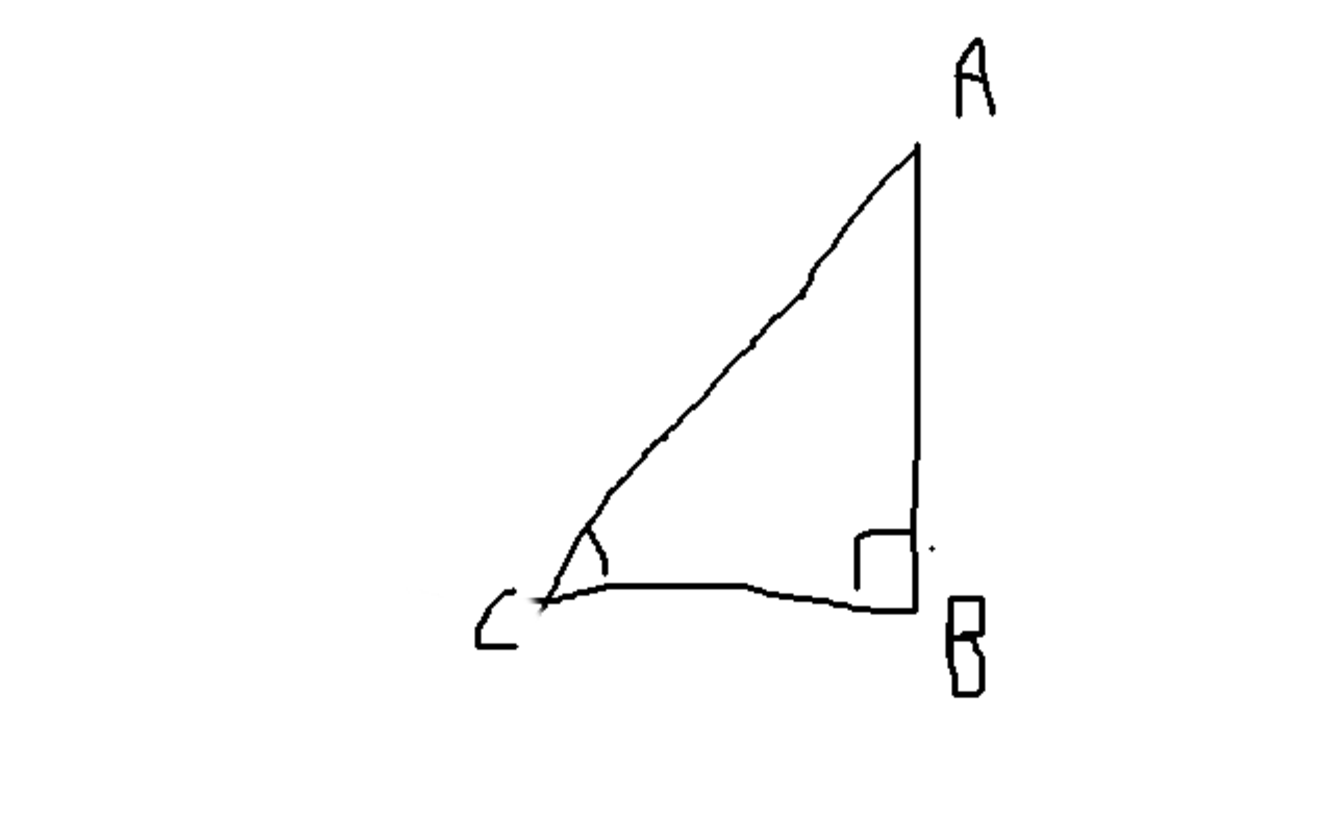
\includegraphics[width=5cm]{faux_ex_adj.pdf}
    \end{center}
    le cosinus de l'angle \( \widehat{ACB}\) est le nombre
    \begin{equation}
        \cos(\widehat{ACB})=\frac{ CB }{ CA }.
    \end{equation}
\end{example}


% This is part of Un soupçon de mathématique sans être agressif pour autant
% Copyright (c) 2015
%   Laurent Claessens
% See the file fdl-1.3.txt for copying conditions.

%--------------------------------------------------------------------------------------------------------------------------- 
\subsection*{Activité : un toboggan pas trop incliné}
%---------------------------------------------------------------------------------------------------------------------------

\begin{enumerate}
    \item
        Un concepteur de toboggan aquatique veut en faire un particulièrement raide : une descente de \SI{5}{\meter} de long avec un angle de \SI{52}{\degree} avec l'horizontale. À quelle hauteur doit commencer la descente ?
    \item
        Un concepteur de jeu pour enfant veut créer un toboggan dont la longueur sera de \SI{3}{\meter} pour un dénivelé (vertical) de \SI{1.5}{\meter}. Quel sera l'angle de descente ?
\end{enumerate}



%+++++++++++++++++++++++++++++++++++++++++++++++++++++++++++++++++++++++++++++++++++++++++++++++++++++++++++++++++++++++++++ 
\section{Calculatrice}
%+++++++++++++++++++++++++++++++++++++++++++++++++++++++++++++++++++++++++++++++++++++++++++++++++++++++++++++++++++++++++++

\begin{Aretenir}
    Pour savoir le cosinus d'un angle, il y a la touche \info{cos} de la calculatrice. Pour savoir l'angle dont le cosinus est donné, il y a la touche \info{cos\^{}-1}.
\end{Aretenir}

Afin de vérifier si la calculatrice est en degré, vérifier que \( \cos(90)\) est bien égal à \( 0\). En radian elle donne environ \( -0.448\).

